\section{二次函数与几何}



\subsection{二次函数的几何变换}

\subsubsection*{平移}
还记得平移运动吗?简单回顾:平移是全等的几何变换(平移前和平移后的图形全等),平移具有交换性(比如一个正方形先向上平移3个单位再向左平移3个单位,如果颠倒顺序,最终位置相同)和可逆性(平移后可以通过反向平移回到原位置).
\par
对二次函数平移其实就是\textbf{对二次函数的顶点平移},进行任何平移操作前需要先把二次函数化为顶点式以方便操作.
\par
假设有\(y=a(x-h)^2\),若\(h>0\)则函数向左平移,若\(h<0\)则函数向右平移,都是平移\(|h|\)个单位;假设有\(y=ax^2+k\),若\(k>0\)则函数向上平移,若\(k<0\)则函数向下平移,都是平移\(|k|\)个单位.两者一起进行就是顶点式\(y=a(x-h)^2+k\).
\par
由于

\begin{example}抛物线\( l_1 \)是由抛物线\( l_2 \)向下平移3个单位长度,再向左平移2个单位长度得到的,已知抛物线\( l_1 \)的解析式为\( y=2(x-2)^2+3 \),则抛物线\( l_2 \)的解析式为(\hspace{3.5em})

\begin{enumerate}[label=\Alph*.]
    \item \( y=2(x-4)^2+6 \)
    \item \( y=2(x-2)^2 \)
    \item \( y=2x^2+6 \)
    \item \( y=2x^2 \)
\end{enumerate}
\end{example}
\begin{solution}
    分析:因为1由2向下平移3个单位再向左平移2个单位,题目已知1求2,只需对1进行反向操作,即向右平移2个单位再向上平移3单位,经过计算A正确.
\end{solution}
以上是抛物线沿坐标轴方向平移的例子,如果沿斜向(即直线)平移呢?这时候只要知道平移的距离和直线的解析式,过移动后的顶点做垂线,垂直于坐标轴,就能\textbf{构造一个直角三角形}.根据直线解析式,\textbf{设移动后顶点的坐标},顶点的横纵坐标值就是三角形直角边的长,最后通过\textbf{勾股定理}就能得出移动后顶点的坐标.
\begin{example}
    将抛物线 \( y = x^2 \) 沿直线 \( y = 3x \) 方向移动 \(\sqrt{10}\) 个单位长度,若移动后抛物线的顶点在第一象限,则移动后抛物线的解析式是\underline{\hspace{4em}}。
\end{example}
\begin{solution}
    分析:该二次函数沿一条直线移动,没有指定移动的方向,但题目要求移动后二次函数的顶点在第一象限,因为该直线(正比例函数)的斜率为\(3>0\),\(x>0\)时\(y\)随\(x\)的增大而增大,所以只有在二次函数往右上方移动时才符合题意(可以画草图辅助理解,如图\ref{fig:move1}),此时根据正比例函数可以设移动后的坐标为\((m,3m)\),再作\(BA\)垂直于\(x\)轴,原点为点\(C\),移动后的定点坐标为\(B\),\(BA=3m,CA=m,CB=\sqrt{10}\),利用勾股定理即可求出移动后的顶点坐标,根据顶点坐标列成顶点式再化为一般式即可.
    \par
    \begin{figure}[h]
        \centering
    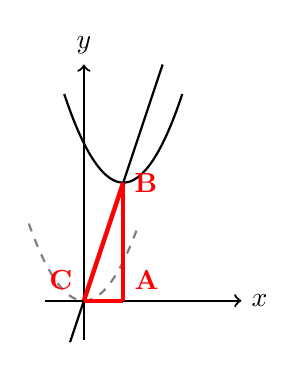
\begin{tikzpicture}[scale=0.5]
    % 绘制坐标系
                                        \draw[->, thick] (-1,0) -- (4,0) node[right] {$x$}; % x轴
                                        \draw[->, thick] (0,-1) -- (0,6) node[above] {$y$}; % y轴
                                        \draw[domain=-1.4:1.4, smooth, dashed, thick, gray] plot (\x, {\x*\x}); % 标注函数
                                        \draw[domain=-0.35:2, smooth, thick] plot (\x, {\x*3}); % 标注函数
                                        \draw[domain=-0.5:2.5, smooth, thick, black] plot (\x, {(\x - 1)^2 + 3}); % 标注函数
                                        \draw[red, ultra thick] (0,0) node[above left] {$\textbf{C}$} -- (1,3) node[right] {$\textbf{B}$};
                                        \draw[red, ultra thick] (1,0) node[above right] {$\textbf{A}$} -- (1,3);
                                        \draw[red, ultra thick] (0,0) -- (1,0);
    \end{tikzpicture}
    \caption{}
        \label{fig:move1}
    \end{figure}
\end{solution}
\begin{exercise}
    \small
    \setlength{\parindent}{0pt} % 取消段落缩进
    \setlength{\columnseprule}{0.01pt}
    \begin{multicols}{2}
    (1)如图1,在平面直角坐标系中,已知点 \( A \) 坐标为 \((2,4)\),直线 \( x=2 \) 与 \( x \) 轴相交于点 \( B \),连接 \( OA \),二次函数 \( y=x^2 \) 图象从点 \( O \) 沿 \( OA \) 方向平移,与直线 \( x=2 \) 交于点 \( P \),顶点 \( M \) 到 \( A \) 点时停止移动。
    %\begin{figure}[h]
        %\centering
        
    %\end{figure}
    \begin{enumerate}
        \item 求线段 \( OA \) 所在直线的函数解析式.
        \item 设二次函数顶点 \( M \) 的横坐标为 \( m \),当 \( m \) 为何值时,线段 \( PB \) 最短,并求出二次函数的解析式.
        \item 当线段 \( PB \) 最短时,二次函数的图象能否过点 \( Q(a,a-1) \) ? 若能,求出 \( a \) 的值;若不能,请说明理由.
    \end{enumerate}




    (2)已知抛物线 \( y = ax^2 - 2ax - 8 \ (a \neq 0) \),若将该函数先向左平移 1 个单位,再向上平移 9 个单位,顶点恰好落在原点上。

    \begin{enumerate}
        \item 求抛物线的函数解析式和顶点坐标;
        \item 若有一直线 \( l \) 与抛物线交于点 \( A(-3, m) \),\( B(n, 16) \),且 \( n > 0 \)。若点 \( P \) 在抛物线上且在直线 \( l \) 下方,且点 \( P \) 不与点 \( A, B \) 重合,分别求出点 \( P \) 横坐标与纵坐标的取值范围。
    \end{enumerate}
    
    \end{multicols}

    
\begin{figure}[h]
                \subfigure{
                        \begin{minipage}{5cm}
                                \centering
                                        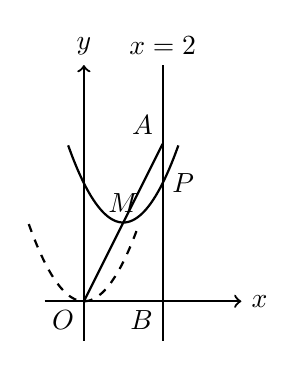
\begin{tikzpicture}[scale=0.5] % 整体缩放
                                        % 绘制坐标系
                                        \draw[->, thick] (-1,0) -- (4,0) node[right] {$x$}; % x轴
                                        \draw[->, thick] (0,-1) -- (0,6) node[above] {$y$}; % y轴
                                        % 标注原点 O
                                        \node at (0,0) [below left] {$O$};
                                        % 绘制点 A(2,4)
                                        \filldraw (2,4) circle (0pt) node[above left] {$A$};
                                        % 绘制直线 x=2(虚线)
                                        \draw[thick] (2,-1) -- (2,6) node[above] {$x=2$};
                                        % 绘制点 B(2,0)
                                        \filldraw (2,0) circle (0pt) node[below left] {$B$};
                                        % 绘制直线 OA(实线)
                                        \draw[thick] (0,0) -- (2,4) node[midway, above left, black] {}; % 不额外标注
                                        % 绘制初始二次函数 y=x^2(虚线,示意原始位置)
                                        \draw[domain=-1.4:1.4, smooth, dashed, thick] plot (\x, {\x*\x}); % 标注函数
                                        % 绘制平移后的二次函数(示例:顶点 M 在 (1,2) 处)
                                        % 函数解析式:y = (x-1)^2 + 2 = x^2 - 2x + 3
                                        \draw[domain=-0.4:2.4, smooth, thick] plot (\x, {(\x-1)^2 + 2}); % 标注
                                        % 标注顶点 M(1,2)
                                        \filldraw (1,2) circle (0pt) node[above] {$M$};
                                        % 标注点 P(2,3)(二次函数与 x=2 的交点)
                                        \filldraw (2,3) circle (0pt) node[right] {$P$};
                                        
                                        \end{tikzpicture}
                                        \par
                                        图1
                        \end{minipage}
                }
\end{figure}
\end{exercise}













\subsubsection*{轴对称}
\subsection{二次函数与\textbf{线段}}

\subsubsection*{线段值}

\subsubsection*{线段关系}

\subsubsection*{线段最值}

\subsection{二次函数与\textbf{面积}}

\subsubsection*{面积公式与割补}

\subsubsection*{铅锤法}

\subsubsection*{转化法}

\subsection{二次函数与\textbf{角度}}

\subsubsection*{角度定值或范围}

\subsubsection*{角度数量关系}

\subsection{二次函数与\textbf{特殊几何图形}}

\subsubsection*{特殊三角形}

\subsubsection*{特殊四边形}